\chapter{Liouville Geometry for Dissipative Systems}
\label{chap:contact_mechanics}
The contact-geometric counterpart of Hamiltonian and Lagrangian mechanics has been the subject of increasing academic interest in recent years, see for example \citet{VanderSchaft2021a,VanderSchaft2018,Maschke2018,Bravetti2017,DeLeon2020}, etc. The conception of the idea arguably traces back to the work of Herglotz \cite{Guenther1996}, who derived it using the variational principle, and the developments in differential geometry, by e.g. \citet{Arnold1989} and \citet{Libermann1987}.

In this chapter, the direct connection is made between the Caldirola-Kanai Hamiltonian given by \cref{eq:ham_CK} and the contact Hamiltonian described by \citet{Bravetti2017}, using Liouville geometry\footnote{It is interesting to note that Bravetti gives the Caldirola-Kanai method as an example of dissipative Hamiltonians in his paper, but fails to make the connection with his own method.}. We then proceed to \emph{contact Lagrangian mechanics}, strongly related to the Herglotz' work. Finally, the whole theory is explained from a thermodynamic perspective as well. While it was already known for some time (dating back to Arnol'd) that contact geometry is the preferred geometry for thermodynamics, its equivalence to contact geometry in (dissipative) classical mechanics has not been desribed in past literature. This underpins a famous statement by Vladimir Arnol'd that `contact geometry is all geometry', in the sense that conservative mechanical systems can be considered as part of a larger class of systems for which energy dissipation \emph{is} allowed. \cite{Geiges2008}

The traditional picture is that Hamiltonian mechanics takes place in the space of generalized positions and momenta, colloquialy denoted by $q$'s and $p$'s. The generalized positions form coordinates of the configuration manifold, which encodes all the possible positions that the system can find itself in. The momenta, on the other hand, are \emph{cotangent variables}: they live in the cotangent space of linear functions acting on tangent (velocity) vectors to the configuration manifold $Q$. We say that the Hamiltonian is a function on the \emph{cotangent bundle} to the configuration manifold $\ctbundle{Q}$. This cotangent bundle has a canonical `symplectic' structure, given by its symplectic form $\omega$, that pairs every position direction with its corresponding momenta:
$$ \omega = \sum \wedgep{\dd{q^i}}{\dd{p_i}}. $$
A vital property of symplectic manifolds (which include the cotangent bundle) is the fact that they are always even-dimensional: every position coordinate has a corresponding momentum and vice versa. Likewise, in an economic context this asserts that every product has its own price. It is precisely this symmetry that is broken by the introduction of contact manifolds.

The symplectic structure of Hamiltonian mechanics is related to the conservation of energy principle, The Hamiltonian function is conserved along the integral curves of the Hamiltonian vector field that it generates. For dissipative mechanics, this strict reciprocity between position and momentum is broken. Either, one constructs an explicit time-dependence and acknowledges the special nature of time, or one can introduce another coordinate that acts as `reservoir' to facilitate the dissipation in the system. These Hamiltonian systems are known as \emph{contact Hamiltonian systems}. One of the contributions of this thesis is to show how both methods are essentially equivalent, by connecting the most famous time-dependent model by Caldirola and Kanai to the contact Hamiltonian by \citet{Bravetti2017}.

\begin{figure}[ht!]
    \begin{center}
        \begin{tikzpicture}[every node/.style={outer sep=0pt,thick}]
    \tikzstyle{spring}=[thick,decorate,decoration={zigzag,pre length=0.3cm,post length=0.3cm,segment length=6}]
    \tikzstyle{damper}=[thick,decoration={markings,  
      mark connection node=dmp,
      mark=at position 0.5 with 
      {
        \node (dmp) [thick,inner sep=0pt,transform shape,rotate=-90,minimum width=15pt,minimum height=3pt,draw=none] {};
        \draw [thick] ($(dmp.north east)+(2pt,0)$) -- (dmp.south east) -- (dmp.south west) -- ($(dmp.north west)+(2pt,0)$);
        \draw [thick] ($(dmp.north)+(0,-5pt)$) -- ($(dmp.north)+(0,5pt)$);
      }
    }, decorate]
    \tikzstyle{ground}=[fill,pattern=north east lines,draw=none,minimum width=0.75cm,minimum height=0.3cm]

    \node (M) [draw,minimum width=1cm, minimum height=1.5cm] {$m$};

    \node (ground) [ground,anchor=north,yshift=-0.25cm,minimum width=1.5cm] at (M.south) {};
    \draw (ground.north east) -- (ground.north west);
    \draw [thick] (M.south west) ++ (0.2cm,-0.125cm) circle (0.125cm)  (M.south east) ++ (-0.2cm,-0.125cm) circle (0.125cm);

    \node (wall) [ground, rotate=-90, minimum width=2cm,yshift=-3cm] {};
    \draw (wall.north east) -- (wall.north west);

    \draw [spring] (wall.160) -- ($(M.north west)!(wall.160)!(M.south west)$) node[pos=0.5,anchor=south, outer sep=4pt] {$k$};
    \draw [damper] (wall.20) -- ($(M.north west)!(wall.20)!(M.south west)$) node[pos=0.5,anchor=north, outer sep=10pt] {$b$};

    \path (wall) ++(0.1cm, 1.2cm) -| node (q) {} (M);
    \draw[|->] (wall) ++(0.2cm, 1.2cm) -- (q.center) node[pos=0.5, anchor=south] {$q$};
    \draw (q) ++(0, 0.1cm) -- ++(0, -0.5cm);

    \node[bgelement] (J1) at (4.5, -1) {1};
    \node[bgelement, label=north:$k$] (C) at (4.5, 0.5) {C};
    \node[bgelement, label=east:$m$]  (I) at (6, -1) {I};
    \node[bgelement, label=west:$b$]  (R) at (3, 0.5) {R};

    % test
    \draw[bonds] 
        (J1) edge[e_out] (I)
        (J1) edge[f_out] (R)
        (J1) edge[f_out] (C);


\end{tikzpicture}

    \end{center}
    \caption{Schematic of the mass-spring-damper system.}
    \label{fig:dho}
\end{figure}
This chapter (and the application in the following chapter) is primarily concerned with the prototypical dissipative mechanical system: the linearly damped harmonic oscillator depicted in \cref{fig:dho}, with the governing second-order differential equation being
\begin{equation}  
  m\ddot{q} + b\dot{q} + kq = 0.
\end{equation}
The choice for this system is rather perspicuous, since it is arguably the `easiest' dissipative system that also exhibits second-order dynamics and is linear in all terms. Furthermore, as discussed below, it serves as the test case of choice in the overwhelming majority of research into dissipative Lagrangian and Hamiltonian mechanics
\cite{Dekker1981,Hutters2020b}. However, the method described in this section can be generalized directly to a general (possibly time-dependent) potential function $V = V(q, t)$. To make calculations and notation easier, some special parameters are frequently used throughout this chapter, they are summarized in \cref{tab:dho_params}.

\begin{table}[ht!]
    \caption{Parameter conventions of the damped harmonic oscillator. To avoid confusion with the symplectic form $\omega$, angular frequencies are denoted by $\Omega$ instead of the conventional lower case Greek letter.}
    \label{tab:dho_params}
    \begin{center}
        \begin{tabular}{llll}
            \toprule
            \textbf{Name} & \textbf{Symbol} & \textbf{Value} & \textbf{Units} \\
            \midrule
            Damping coefficient & $\gamma$ & $b/m$ & \si{\per \second }\\[0.4cm]
            Undamped frequency & $\Omega_o$ & $\sqrt{k/m}$ & \si{\per \second }\\[0.4cm]
            Damped frequency & $\Omega_d$ & $\sqrt{\Omega_0^2 - \qty(\frac{\gamma}{2})^2}$ & \si{\per \second }\\[0.4cm]  
            Damping ratio & $\zeta$ & $\frac{b}{2\sqrt{mk}}$ & -- \\[0.2cm]
            \bottomrule
        \end{tabular}
    \end{center}
\end{table}

\section{The Caldirola-Kanai method}
\label{sec:caldirola}
A traditional, engineering-inclined method to incorporate damping in the framework is to include a Rayleigh damping term in the Lagrangian to emulate linear damping forces, and this works `mathematically' to derive the correct equations of motion \cite{Goldstein2011}. Although frequently used for practical problems, this damping term is not really part of the \emph{actual} Lagrangian --- rather, it simply makes use of the notion of a generalized force that is not inherently part of the system. As such, this method only works on a superficial level: the pristine differential geometric foundations of mechanics do not leave room for such ad hoc tricks. There is, as a result, also no Hamiltonian counterpart for this method. 

The historical attempts to do better than the Rayleigh method were primarily motivated by the application of the (dissipative) Hamiltonian formalism in quantum mechanics through discretization. For this application, a sound mathematical structure is of the essence, which calls for a more rigorous approach. A celebrated paper by
\citet{Dekker1981} provides an excellent summary of many attempts up to 1981. Indeed, the well-studied approach developed by \citet{Caldirola1941} and \citet{Kanai1948} was intended exactly for this purpose. This method features an explicit time-dependence both in the Lagrangian function
\begin{equation}
    \Lck(q, \dot{q}, t) = \ec^{\gamma t}\qty(\frac{1}{2}m\dot{q}^2 - \frac{1}{2}kq_1^2),
    \label{eq:lag_CK}
\end{equation}
and the corresponding Hamiltonian function:
\begin{equation}
    \Hck(q, \Pcan, t) = \frac{\Pcan^2}{2m}\ec^{-\gamma t} + \frac{1}{2}kq^2\ec^{\gamma t}.
    \label{eq:ham_CK}
\end{equation}
In latter equation, $\Pcan$ refers to a special `canonical momentum', that is
\begin{equation}
    \Pcan \equiv \pdv{\Lck}{\dot{q}},
    \label{eq:can_momentum}
\end{equation}
which is related to the `true` kinematic momentum by the relation $\Pcan = p\ec^{\gamma
t} = m\dot{q}\ec^{\gamma t}$. As such, it is also clear that the Caldirola-Kanai Lagrangian and Hamiltonian functions are related by the Legendre transform \emph{with respect to the canonical momentum}:
%\footnote{The `Legendre transform'
%refers, in the context of fiber bundles, to the so-called fiber derivative. On a manifold $M$, let $L \in
%\functions{M}$. Then the fiber derivative is defined als 
%    $$ \fiberder{L}: \tbundle{L}\to\ctbundle{L}: \fiberder{L}(\vec{v})\cdot\vec{w} = \left. \dv{}{s}\right\vert_{s = 0} L(\vec{v} +
%    s\vec{w}). $$
% Hence, the Legendre transform is in the first place the mapping that associates the generalized velocities with the
% associated (canonical) generalized momenta. Importantly, this mapping is a diffeomorphism (that is, invertible and onto) if the Hessian of
% $L$ is nondegenerate - roughly equivalent to the statement that every generalized velocity has an associated `mass` to
% it. \cite{Marsden1998}}
$$ \Hck = \Pcan \dot{q} - \Lck. $$
From either \cref{eq:lag_CK} or \cref{eq:ham_CK}, the equations of motion are readily
derived (for the Hamiltonian case with respect to $\Pcan$ after which the transformation to $p$ can be effected).
Indeed, after taking the appropriate derivatives, one obtains:
\begin{equation*} 
    \begin{split}
        \dv{}{t}\qty(\pdv{\Lck}{\dot{q}}) - \pdv{\Lck}{q} &= 0 \\
        \Rightarrow \ec^{\gamma t}\qty(m\ddot{q} + m\gamma\dot{q} + kq) &= 0
    \end{split}
\end{equation*}
for the Lagrangian case. Likewise, Hamilton's equations yield: \cite{Tokieda2021}
\begin{equation*}
    \begin{split}
        \dot{q} &= \pdv{\Hck}{\Pcan} = \frac{\Pcan}{m}\ec^{-\gamma t} =  \frac{p}{m}, \\
        \dot{\Pcan} &= -\pdv{\Hck}{q} = -kq\ec^{\gamma t}.\\
    \end{split}
\end{equation*}
The relation between the time derivatives of the momenta $\dot{p}_1$ and $\dot{\Pcan}$ is slightly more involved since one must invoke the product rule as a result of their time-dependent relation:
    $$ \dot{\Pcan} = \ec^{\gamma t}\qty(\dot{p}_1 + \gamma p). $$
Substition yields the correct equation for $p$, though the equation is again multiplied by $\ec^{\gamma t}$. Because the latter is sufficiently well-behaved (that is, it has no zeros), it can be removed without any problems.

\paragraph{Geometric perspective}
To put the above derivation in a geometric setting, define the Liouville 1-form as
$$ \alpha = \Pcan\dd{q} \quad \Rightarrow \quad \omega = -\dd{\alpha} = \wedgep{\dd{q}}{\dd{\Pcan}},$$
where the symplectic 2-form will be used to obtain Hamilton's equations. The Hamiltonian \cref{eq:ham_CK} is explicitly time-dependent. This will give rise to a time-dependent vector field governing the solution curves.\footnote
{A \emph{time-dependent vector field} on a manifold $M$ is a mapping $X: M\times\real \to \tbundle{M}$ such that for each $t \in \real$, the restriction $X_t$ of $X$ to $M \times \{t\}$ is a vector field on $M$. \cite{Libermann1987} An additional construction of importance, called the \emph{suspension} of the vector field, is a mapping $$ \tilde{X}: \real \times M \to \tbundle{(\real \times M)} \quad (t, m) \mapsto ((t, 1), (m, X(t, m))),$$ that is to say, it lifts the vector field to the extended space that also includes $t$ and assigns the time coordinate with a trivial velocity of 1. \cite{Abraham1978}}
The construction of the vector field associated with a time-dependent Hamiltonian follows the same construction rules as a normal Hamiltonian (using the isomorphism given by $\omega$), but `frozen' at each instant of $t$. Even more bluntly speaking, one simply ignores the $t$-coordinate during the derivation, only to acknowledge the dependence at the very end. This leads to the following vector field, `suspended' on the $\real\times Q$ space:
$$ \tilde{X}_{\Hck} = -\ec^{\gamma t}kq\pdv{}{\Pcan} + \ec^{-\gamma t}\frac{\Pcan}{m}\pdv{}{q} + \pdv{}{t}.$$
The suspension is important to make the final coordinate transform from $\rho$ to $p$ work properly. Indeed, effecting the transformation $(q, \Pcan, t) \mapsto (q, \ec^{-\gamma t}\Pcan, t)$, one obtains
$$ \tilde{X}_{\Hck} = \qty(-kq - \gamma p)\pdv{}{p} + \frac{p_1}{m}\pdv{}{q} + \pdv{}{t}.$$
It is worthwile to ponder on some apparent peculiarities in the Caldirola-Kanai method, for they will be explained elegantly by the contact-Hamiltonian formalism. Firstly, the role of the two-different momenta is not very clear from the get-go, apart from being a consequence of the way the Caldirola-Kanai Lagrangian is formulated. This has also been the reason for considerable confusion in the academic community (see \citet{Schuch1997}). Furthermore, there is the special role of the time coordinate, which is merely a parameter in the Hamiltonian function; for it does not partake in the dynamics of the system. Finally, there is the special role of the factor $\ec^{\gamma t}$ through which the time-dependence makes its appearance both in the Lagrangian and the Hamiltonian.

%\section{Symplectification and Liouville structures}
%We start with an $n$-dimensional \emph{base manifold} $Q$. In the context mechanical systems, this manifold is the configuration manifold of the system, \emph{extended} with an additional, `special` position coordinate coordinate that will be interpreted later. Let us assume that $Q$ has coordinates $\vec{q} = \qty(q_0, q, \ldots, q_n)$. For the damped harmonic oscillator, this manifold is two-dimensional, for it contains just the special coordinate and the position of the mass. Without loss of generalization, we will denote the special position coordinate by $q_0$.
%
%Now, introduce the \emph{manifold of contact elements} $\cbundle{Q}$, to the base manifold $Q$. This is the manifold of all points in $Q$, with the space of all possible tangent hyperplanes at every point. This manifold has dimension $2n-1$.
%
%The manifold of contact elements to $Q$ can be identified with the projectivization of the cotangent bundle $\ctbundle{Q}$, denoted by $\pctbundle{Q}$. This manifold is of dimension $2n-1$. 

\section{From time-dependent to contact Hamiltonian systems}
In the subsequent discussion the original Hamiltonian will be progressively lifted to higher-dimensional spaces in order to include dissipation in the Hamiltonian formalism. First of all, to a contact manifold, which is odd-dimensional: as mentioned, we need an additional degree of freedom --- which has no momentum conjugate to it --- to keep track of the dissipation in the system. This degree of freedom is sometimes referred to as a \emph{gauge variable}, denoted by $q_0$.  However, performing calculations in contact geometry directly is cumbersome and uninsightful: to quote Vladimir Arnol'd once more, `one is advised to calculate symplectically but to think rather in contact geometry terms'. Hence, we make use of the \emph{symplectization} of the contact structure, which gives rise to a so-called \emph{Liouville structure}, and `pretend' that we are dealing with the symplectic case. This symplectization will add yet another dimension to the system. \cite{VanderSchaft2021a,Arnold1989a}

\subsection{Symplectization \& Liouville structures}
The contact manifold of our system is three-dimensional, with coordinates $p, q$ and $q_0$ -- the latter is the gauge variable for the dissipation in the system. It can be viewed as the manifold of contact elements associated with the extended configuration manifold $M$ for which $q$ and $q_0$ are coordinates, denoted by $\pctbundle{M}$. The contact form on $\pctbundle{M}$ is given by 
\begin{equation}
    \alpha = \dd{q}_0 - p\dd{q},
    \label{eq:dho_contact_form}
\end{equation}
which accentuates the special role of the $q_0$ in the system dynamics. Contact forms are, by their very nature, ambiguous, for they represent a distribution of hyperplanes, which coincides with the kernel of the 1-form. Multiplication with a nonzero factor yields a different form with the same kernel, that is to say, they represent the same contact structure. This is the reason behind the `projective' nature of contact mechanics\footnote{As explained in \cref{app:contact_geometry}, the manifold of contact elements is bundle-isomorphic to the projectivization of the cotangent bundle.}. Hence, one may just as well multiply the 1-form with a nonzero factor $\lambda$:
$$ \lambda\qty(\dd{q}_0 - p\dd{q}) \quad \lambda \in \real_0. $$
The factor $\lambda$ can be considered to be an extra degree of freedom (leaving the contact structure unaffected), which provides a `lift' from the odd-dimensional manifold to an even-dimensional one, which is called the symplectification of the contact manifold. \cite{Arnold1989}

More formally, introduce the \emph{principal} $\mgroup$-bundle $\bundle{\ctzbundle{M}}{\pi}{\pctbundle{M}}$, where $\mgroup$ acts in the fiber through `dilations' of the fiber which amounts to an equal scaling of all the cotangent variables (this is the multiplication by $\lambda$ in the above expression). Here, $\ctzbundle{M}$ is the cotangent bundle to $M$, but with the zero section removed --- this is required for the group to act freely. This principal bundle $\bundle{\ctzbundle{M}}{\pi}{\pctbundle{M}}$ admits what is called a \emph{fibered symplectic Liouville structure}, given by the Liouville form \cite{Libermann1987}
$$ \theta = \lambda ( \dd{q_0} + p \dd{q} ). $$
To restate the above in canonical coordinates, choose
\begin{equation}
    \rho_0 = \lambda \quad \text{and} \quad \rho = -\lambda p
    \label{eq:homo_coords}
\end{equation}
such that
\begin{equation} 
    \theta = \rho_0\dd{q}_0 + \rho\dd{q}, 
    \label{eq:dho_liouville_form}
\end{equation}
which is the Liouville form on $\ctbundle{M}$. \cite[p. 308]{Libermann1987}  The Liouville form defines a symplectic structure given by\footnote
{The nondegeneracy condition on the contact structure guarantees that this structure is indeed symplectic.}
$$\omega = -\dd{\theta} = \wedgep{\dd{q_0}}{\dd{\rho_0}} + \wedgep{\dd{q}}{\dd{\rho}}.$$ 
The manifold $\ctzbundle{M}$ is called the symplectization of the contact manifolds, and consists of all four-tuples $(q_0, q, \rho_0, \rho)$ for which $\rho_0$ and $\rho$ do not simultaneously vanish. For now, we have not assigned any specific meaning to the coordinates given above, but they will turn out to match with the notation used in \cref{eq:lag_CK,eq:ham_CK}, etc.
\begin{figure}[h!]
    \begin{center}
        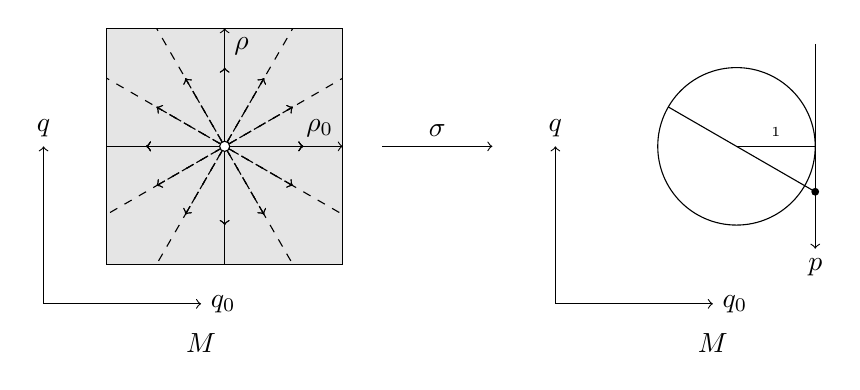
\begin{tikzpicture}
    \draw[->] (0, 0) -- (2, 0) node[anchor=west] {$q_0$};
    \draw[->] (0, 0) -- (0, 2) node[anchor=south] {$q$};
    
    \node (m) at (2.3, 2) {};
    
    \filldraw[draw=black, fill=gray!20] (m) ++(-1.5, -1.5) -- ++(0, 3) -- ++(3, 0) -- ++(0,-3) -- cycle;
    \draw[->] (m) ++(-1.5, 0) -- ++(3, 0) node[anchor=south east] {$\rho_0$};
    \draw[->] (m) ++(0, -1.5) -- ++(0, 3) node[anchor=north west] {$\rho$};
        
    \begin{scope}
        \clip (m) ++(-1.5,-1.5) rectangle ++(3, 3);
        \foreach \i in {0,30,...,180}{
            \draw[<->, dashed] (m) ++({-cos(\i)}, {-sin(\i)}) -- ++({2*cos(\i)}, {2*sin(\i)});
        }
        \foreach \i in {0,30,...,180}{
            \draw[<->, dashed] (m) ++({-cos(\i)}, {-sin(\i)}) -- ++({2*cos(\i)}, {2*sin(\i)});
        }
        \foreach \i in {0,30,...,180}{
            \draw[dashed] (m) ++({-4*cos(\i)}, {-4*sin(\i)}) -- ++({8*cos(\i)}, {8*sin(\i)});
        }
    \end{scope}
    
    \node[circle,draw=black,fill=white,inner sep=1.3pt] at (m) {};
    
    \draw[->] (6.5, 0) -- (8.5, 0) node[anchor=west] {$q_0$};
    \draw[->] (6.5, 0) -- (6.5, 2) node[anchor=south] {$q$};
    
    \node[fill=none] (m2) at (8.8, 2) {};
    
    \draw (m2) circle (1);
    \draw[->] (m2) ++(1, 1.3) -- ++(0, -2.6) node[anchor=north] {$p$} ;
    \draw (m2.center) ++(-0.866, 0.5) -- (9.8, 1.423) node[circle,fill=black, inner sep = 1pt] {};
    \draw (m2.center) -- ++(1, 0) node[pos=0.5,anchor=south] {\tiny{1}};
    %\draw[->] (m) ++(-1.5, 0) -- ++(3, 0) node[anchor=west] {$\rho_0$};
    %\draw[->] (m) ++(0, -1.5) -- ++(0, 3) node[anchor=south] {$\rho$};
    
    \draw[->] (4.3, 2) -- (5.7, 2) node[pos=0.5,anchor=south] {$\sigma$};
     
    \node at (2, -0.5) {$\ctzbundle{M}$};
    \node at (8.5, -0.5) {$\pctbundle{M}$};
\end{tikzpicture}

    \end{center}
    \caption{Illustration of the principal $\mgroup$-bundle $\bundle{\ctzbundle{M}}{\pi}{\pctbundle{M}}$. The total space $\ctzbundle{M}$ is the cotangent bundle to $M$ with zero section removed, which is shown on the left. The action by the multiplicative group $\mgroup$ is illustrated by the arrows, for it acts as a scaling (dilation) on all the cotangent variables. The origin is not part of the fiber, for it is part of the zero section. The bundle projection $\pi$ projects all points that are on the same orbit (straight lines through the origin) to a single point on the base manifold: the projectivized cotangent bundle $\pctbundle{M}$. The former space has a symplectic structure while the latter space has a contact structure. Observe from \cref{eq:homo_coords} that $p = \rho/\rho_0$, i.e. such that $p$ is a coordinate for the projectivization by stereographic projection, as shown on the right.}
    \label{fig:principal_bundle}
\end{figure}

Finally, the \emph{Liouville vector field} $Z$ associated with the Liouville structure is the vector field that represents the dilation of the fiber in the symplectization. It is defined as
\begin{equation}
    Z = \raiseIndex{\theta} = \rho_0\pdv{}{\rho_0} + \rho\pdv{}{\rho}. 
    \label{eq:liouville_vf}
\end{equation}
Vector field (components) colinear with the Liouville vector fields are called \emph{vertical}; they represent dissipative action in the system. After the vertical components are removed, they remaining vector field is called \emph{horizontal}.

To summarize, we lifted the original system with symplectic structure $\wedgep{\dd{q}}{\dd{p}}$ to a contact manifold through the addition of a gauge variable $q_0$. We then symplectified the contact manifold to a four-dimensional system, with `positions' $(q_0, q)$ and `momenta' $(\rho_0, \rho)$.

\subsection{Homogeneous Hamiltonian systems} The theoretical construction of the past section serves an important purpose, because it is the symplectified space which is the proper setting for the Caldirola-Kanai Hamiltonian discussed in \cref{sec:caldirola}. Along with the symplectification of the contact structure described in the past section, we can do the same with a contact Hamiltonian system.

There is a one-to-one correspondence between contact Hamiltonians on $\pctbundle{M}$ and a special class of Hamiltonians on the symplectified space $\ctzbundle{M}$. These are the Hamiltonians which are \emph{homogeneous} in the cotangent variables with degree 1:\footnote
{This is a consequence of the Euler theorem for homogeneous functions. If $H = H(\vec{q}, \vec{\rho})$ is homogeneous of degree $r$ in $\vec{\rho}$, then
    $$ \sum_{i = 1}^n \rho_i \pdv{H}{\rho_i} = r H. $$
 Hence for homogeneity of degree 1, we have: 
 $$ \lied{Z}{H} = Z(H) = \sum_{i=1}^n \rho_i \pdv{H}{\rho_i} = H \quad \text{with}\quad Z \equiv \sum \rho_i \pdv{}{\rho_i}. $$
}
\begin{equation}
    H(q_0, q, \lambda \rho_0, \rho) = \lambda H(q_0, q, \rho_0, \rho) \quad \text{or} \quad \lied{Z}{H} = H,
\end{equation}
with $\lambda \in \real_0,\: H \in \functions{\ctzbundle{M}}$ and $Z$ defined according to \cref{eq:liouville_vf}. Given that $H$ is indeed homogeneous of degree 1, this correspondence is in canonical cooridinates:
\begin{equation}
    H(q_0, q_1, \rho_0, \rho_1) = \rho_0 \hat{H}\qty(q_0, q_1, \frac{\rho_1}{\rho_0})
    \label{eq:H_correspondence}
\end{equation}
where $H \in \functions{\ctzbundle{M}}$, $\hat{H} \in \functions{\pctbundle{M}}$ and let $p = \rho_i / \rho_0$ be a coordinate for the projectivized fiber. Likewise, there is also a direct correspondence between the vector fields generated by these Hamiltonians, and therefore the system dynamics. This is the reason why we go through the trouble of symplectification in the first place, because it offers computational advantages. It is possible to derive the contact equations directly (as \citet{Bravetti2017} does), but it does not offer the same amount of insight and as its symplectified counterpart. \cite{VanderSchaft2021a,Arnold1989}

Now, recall the Caldirola-Kanai Hamiltonian. Instead of assuming a direct time-dependence, we will think of the time-dependence as the gauge momentum, i.e. $\rho_0 = \ec^{\gamma t}$. However, we will now consider $\rho_0$ to be a coordinate in its own right, instead of directly using the expression above. The Caldirola-Kanai Hamiltonian is then written as (cf. \cref{eq:ham_CK}):
\begin{equation}
    H: \ctzbundle{M} \to \real: \quad H(q_0, q, \rho_0, \rho) = \rho_0 \qty[\frac{1}{2m}\qty(\frac{\rho}{\rho_0}) + \frac{1}{2}kq^2]. 
    \label{eq:homo_hck}
\end{equation}
The motivation to make this particular choice is twofold: first, observe that $H$ is homogeneous in the cotangent variables $\rho_0, \rho$, and second, that their fraction yields the \emph{real} momentum: $ p = \rho/\rho_0 $. Using the correspondence given by \cref{eq:H_correspondence}, the Hamiltonian may be `projected' to the contact Hamiltonian $\hat{H}$:
\begin{equation}
    \hat{H}: \pctbundle{M} \to \real: \quad \hat{H}(q_0, q, p) = \frac{p^2}{2m} + \frac{1}{2}kq^2.
\end{equation}
Numerically, this contact Hamiltonian is the same as the Hamiltonian for an undamped particle, but it is defined on the contact manifold that also takes into account the gauge variable $q_0$. 



